%default language is German. use the second line instead for english settings:
\RequirePackage{ifpdf}
\documentclass{lni}
%\documentclass[english]{lni}

\IfFileExists{latin1.sty}{\usepackage{latin1}}{\usepackage{isolatin1}}

\usepackage{graphicx}
\usepackage[utf8]{inputenc}

% Extra packages

\usepackage{amsmath}
\usepackage{amssymb}
\usepackage{amsthm}

\usepackage{latexsym}

\usepackage{mathtools}

\usepackage{tikz}
\usetikzlibrary{automata,positioning}

% Own environments

\newtheoremstyle{def_style}
{\topsep}{\topsep}%
{}{}%
{\bfseries}{}%
{\newline}{}%

\theoremstyle{def_style}
\newtheorem{definition}{Definition}[section]

\newtheoremstyle{break}
{\topsep}{\topsep}%
{}{}%
{\bfseries}{}%
{\newline}{}%

\theoremstyle{break}
\newtheorem{example}{Beispiel}

% Own commands

\newcommand{\AU}[2]{\operatorname{A}[#1\operatorname{U}#2]}
\newcommand{\EU}[2]{\operatorname{E}[#1\operatorname{U}#2]}
\newcommand{\UEqual}[4]{#1\operatorname{U}^{\leq #2}_{\geq #3}#4}
\newcommand{\UStrict}[4]{#1\operatorname{U}^{\leq #2}_{> #3}#4}
\newcommand{\paths}[2]{\operatorname{paths}^{#1}_{#2}}


\author{
	Theodor Teslia \\ 
	\\ 
	Informatik 11 -- Embedded Software \\ 
	RWTH Aachen University \\ 
	Aachen, Germany \\ 
	teslia@embedded.rwth-aachen.de\\
	\\
	\textit{Betreuer}\\
	\textit{Robin Mross}\\ %Dies ist der inhaltliche Betreuer. Wer das ist, erfahren Sie noch.
}
\title{\small{Seminar} \\ \vspace{0.5cm} \Large{Eine Logik für das Schlussfolgern über Zeit und Zuverlässigkeit}}

\newcommand{\CTL}{\mathsf{CTL}}
\newcommand{\PCTL}{\mathsf{PCTL}}

\begin{document}
\maketitle

\begin{abstract}
Eine prägnante Zusammenfassung des Kerninhaltes ohne thematische Einleitung und Fazit. Was ist $\PCTL$ und welche Probleme kann es lösen, die andere Logiken bisher nicht erfüllen konnten.
\end{abstract}

\section{Einführung}

Hier führe ich in die Logik $\PCTL$ ein, die Probleme die diese löst und wie dies circa gemacht wird.
Falls es funktioniert, führe ich außerdem in Halbringsemantik ein und erkläre kurz, in welchem Punkt sich die Ansätze ähneln und unterscheiden.

\section{Grundlagen}
\label{ChapGrundlagen}

Um Erweiterungen einer Logik zu verstehen ist es ratsam die Grundlegende auch zu kennen. Aus diesem Grund soll in diesem Kapitel in die Logik \textit{Computation Tree Logic} ($\CTL$) und naheliegende, wichtige Themen eingeleitet werden.

$\CTL$ ist eine temporale Logik um Aussagen in nicht-deterministischen Systemen zu treffen. 
Dafür betrachtet man Kripkestrukturen, welche eine Art Graph darstellen, da diese viele Eigenschaften liefern, die für $\CTL$-Anwendungsfälle interessant sind.

\begin{definition}[Syntax von $\CTL$]
	Die Menge der $\CTL$-Formeln lässt sich induktiv mithilfe folgender Regeln definieren \cite{clarke1982design, baier2008principles}:
	\begin{enumerate}
		\item Wenn $\mathsf{AP}$ eine Menge an atomaren Aussagen ist, dann ist jedes $a\in \mathsf{AP}$ eine $\CTL$-Formel. Außerdem sind $\top$ und $\bot$ $\CTL$-Formeln.
		\item Wenn $\varphi_1$ und $\varphi_2$ $\CTL$-Formeln sind, dann sind $\neg\varphi_1$, $\varphi_1 \land \varphi_2$ und $\varphi_1 \lor \varphi_2$ ebenfalls $\CTL$-Formeln.
		\item Wenn $\varphi_1$ eine $\CTL$-Formel ist, dann sind auch $\operatorname{EX}\varphi_1$ und $\operatorname{AX}\varphi_1$ $\CTL$-Formeln.
		\item Wenn $\varphi_1$ und $\varphi_2$ $\CTL$-Formeln sind, dass sind $\EU{\varphi_1}{\varphi_2}$ und $\AU{\varphi_1}{\varphi_2}$ auch $\CTL$-Formeln.
	\end{enumerate}
\end{definition}

Bevor die Semantik erläutert wird, sollen zuerst die Strukturen gezeigt werden, die man typischerweise mit $\CTL$ zusammen verwendet.

\begin{definition}[Kripkestrukturen]
	Eine \textit{Kripkestruktur} oder \textit{Transitionssystem} ist ein Graph von der Form $\mathcal{K}=(V, E, \mathcal{L})$, wobei $E$ eine zweistellige Kantenrelation über $V$ ist und $\mathcal{L}$ eine Funktion $\mathcal{L}:V\to2^{\mathsf{AP}}$ ist, die jedem Zustand eine Menge an atomaren Aussagen zuweist 	\cite{clarke1982design,clarke1986automatic}.
	
	Weiter bezeichnen wir einen Pfad als $\sigma=s_0\dots s_n$ mit $s_i\in V$ für alle $i\in\{0,\dots,n\}$ und $\sigma[i]=s_i$ für $0\leq i \leq n$ \cite{baier2008principles}.
\end{definition}

\begin{definition}[Semantik von $\CTL$]
	Für ein Transitionssystem $\mathcal{K}=(V,E,\mathcal{L})$ können wir damit induktiv die Modellbeziehung $\models$ zwischen einem Knoten $v\in V$ und $\CTL$-Formeln definieren \cite{baier2008principles}:
	\begin{enumerate}
		\item $v\models \top \Leftrightarrow \forall x(x=x)$ und $v\models \bot \Leftrightarrow \exists x(x\neq x)$.
		\item Für $a\in \operatorname{AP}$ gilt $v\models a \Leftrightarrow a\in \mathcal{L}(v)$.
		\item Es gilt $v\models \neg \varphi \Leftrightarrow v\not\models \varphi$,\\
		$v\models \varphi_1 \land \varphi_2 \Leftrightarrow v\models \varphi_1 \text{ und } v\models \varphi_2$,\\
		$v\models \varphi_1 \lor \varphi_2 \Leftrightarrow v\models \varphi_1 \text{ oder } v\models \varphi_2$,
		\item Es gilt $v\models \operatorname{EX}\varphi \Leftrightarrow$ es ex. ein $w\in V$ mit $(v,w)\in E$ und $w\models \varphi$ und analog:\\ 
		$v\models \operatorname{AX}\varphi \Leftrightarrow$ für alle $w\in V$ mit $(v,w)\in E$ gilt $w\models \varphi$.
		\item Es gilt $v\models \EU{\varphi_1}{\varphi_2} \Leftrightarrow$ es existiert ein Pfad $\sigma$ in $\mathcal{K}$, der in $v$ beginnt und ein $i\in \mathbb{N}$ so, dass $\sigma[i]\models \varphi_2$ und für alle $0\leq j < i$ gilt $\sigma[i]\models \varphi_1$. 
		Analog ist die Definition für $\AU{\varphi_1}{\varphi_2}$, es muss dann aber für jeden in $v$ beginnenden Pfad ein $i\in \mathbb{N}$ geben so, dass der $i$-te Zustand $\varphi_2$ und alle Zustände davor $\varphi_1$ erfüllen.
	\end{enumerate}
\end{definition}

Intuitiv bedeutet $\operatorname{EX}\varphi$ also, dass $\varphi$ in einem beliebigen Nachfolgezustand gelten muss und $\operatorname{AX}\varphi$, dass $\varphi$ von allen Nachfolgezuständen erfüllt wird.

$\EU{\varphi_1}{\varphi_2}$ bzw. $\AU{\varphi_1}{\varphi_2}$ sagt aus, dass es einen Pfad $\sigma$ gibt bzw. auf allen Pfaden $\sigma$ gilt, dass zuerst $\varphi_1$ gilt, bis von einem Zustand $\varphi_2$ erfüllt wird.
Die anderen Operatoren haben die bekannte Bedeutung.

Um einige Eigenschaften einfacher auszudrücken werden zusätzlich noch weitere Operatoren definiert \cite{clarke1982design}:
\begin{itemize}
	\item $\operatorname{EF}\varphi \equiv \EU{\top}{\varphi}$ und $\operatorname{AF}\varphi \equiv \AU{\top}{\varphi}$ bedeuten intuitiv, dass es einen Pfad gibt bzw. für alle Pfade irgendwann $\varphi$ gilt.
	\item $\operatorname{EG}\varphi \equiv \neg\operatorname{EF}\neg\varphi$ und $\operatorname{AG}\varphi \equiv \neg\operatorname{AF}\neg\varphi$ bedeuten, dass es einen Pfad gibt bzw. für alle Pfade gilt, dass in jedem Zustand $\varphi$ gilt.
\end{itemize}
Mithilfe dieser Syntax und zugehöriger Semantik auf Transitionssystemen lassen sich nun einige interessante Aussagen formulieren:
\begin{example}[Beispiele für $\CTL$-Formeln und deren Bedeutung]
	Sei die Menge der atomaren Aussagen $\mathsf{AP}=\{\mathsf{idle}, \mathsf{error}\}$
	\begin{itemize}
		\item $\operatorname{AG}\operatorname{AF}\mathsf{idle}$ \\ Die Formel gilt für einen Zustand $v$, wenn auf jedem in $v$ beginnenden Pfad, für jeden Zustand auf diesem, irgendwann $\mathsf{idle}$ erfüllt. Das heißt, $\mathsf{idle}$ gilt unendlich oft.
		\item $\operatorname{EF}\operatorname{AG}\mathsf{error}$ \\
		Diese $\CTL$-Formel besagt, dass es einen Pfad gibt, auf dem ab irgendeinem Zustand alle Zustände die atomare Aussage $\mathsf{error}$ erfüllen. Das heißt, es gibt einen Pfad mit einem irreversiblen Fehler.
	\end{itemize}
\end{example}

Zusätzlich soll noch angemerkt werden, dass $0\in \mathbb{N}$ gilt.

\section{Eine Logik für Zeit und Zuverlässigkeit}

% Dieses Kapitel stellt das Hauptkapitel der Arbeit dar und soll die Syntax und Semantik von $\PCTL$ erläutern, sowie mithilfe von eigenen Beispielen diese Verständlicher machen. Offensichtliche verwende ich in dem gesamten Kapitel hauptsächlich \cite{hansson1994logic} für Informationen, Algorithmen und Beweise, die Beispiele werden aber zum Großteil eigene sein.

Wie in Kapitel \ref{ChapGrundlagen} gezeigt, lassen sich mithilfe von $\CTL$ viele interessante Eigenschaften von nicht-deterministischen System beschreiben. 
Jedoch gibt es auch Anwendungsfälle, in denen mehr Ausdruckskraft benötigt wird, als ein All- und Existenzquantor liefern können.
Ein Gebiet in dem dies stark auffällt sind Soft-Realtime Systeme. 
In diesen existieren für Prozesse bestimmte Zeitschranken (\textit{Deadlines}), im Gegensatz zu Hard-Realtime Systemen führt das einhalten einer Zeitschranke aber nicht zu einem Systemabbruch oder katastrophalem Ereignis, sondern stellt beispielsweise nur eine Verschlechterung der Effizienz dar. \cite{hansson1994logic}.
Um eben solche Systeme gut beschreiben zu können benötigt man zwei weitere Aspekte:
\begin{enumerate}
	\item Um die Zeitschranken zu formulieren wird ein Konzept von Zeit benötigt. Dieses soll aussagen können, dass zwei Ereignisse eine bestimmte Zeitspanne $t$ voneinander entfernt sind.
	\item Da aber das Verfehlen einer Zeitschranke nicht unbedingt zum Verwerfen einer Formel führen soll, werden zusätzlich Wahrscheinlichkeiten benötigt. 
	Da in Soft-Realtime Systemen das Überschreiten einer Deadline zwar nicht direkt verboten ist, aber im Allgemeinen vermieden werden sollte, ist es sinnvoll über die Wahrscheinlichkeit eines Ereignisses Aussagen zu treffen.
\end{enumerate}
Kombiniert man diese Aspekte lassen sich Eigenschaften wie \glqq Nach Ereignis X passiert innerhalb von 15 Zeiteinheiten mit Wahrscheinlichkeit 90\% Ereignis Y\grqq{} oder \glqq Ereignis A tritt mit einer Wahrscheinlichkeit von 90\% in 10 und mit 95\% in 20 Zeitschritten auf\grqq. 
Eine Logik, die eben diese Erweiterungen von $\CTL$ sinnvoll implementiert ist die Logik \text{Probabilistic Computation Tree Logic} ($\PCTL$). 
Sinnvoll bedeutet hier, dass es einen Model Checking Algorithmus mit polynomieller Laufzeit gibt. 
In diesem Kapitel soll zuerst die Syntax von $\PCTL$ erläutert werden, danach die dazugehörige Semantik aufgezeigt werden, um dann zwei verschiedene Ansätze für das Model Checking von $\PCTL$ mit Transitionssystemen zu zeigen. 
Im Anschluss sollen die kennengelernten Konzepte der Logik sowie des Model Checkings an einem Beispiel erläutert werden.

\subsection{Syntax und Semantik von $\PCTL$}

Um \textit{Probabilistic Computation Tree Logic} ($\PCTL$) besser zu verstehen, soll hier die Syntax, die Modelle welche wir zum Auswerten verwenden, sowie die Semantik der Logik erläutert werden.

Wie auch für $\CTL$ können wir die Syntax von  $\PCTL$ mithilfe folgender rekursiver Regeln definieren:
\begin{definition}[Syntax von $\PCTL$]
	Die Menge der $\PCTL$-Formeln lässt sich induktiv wie folgt definieren \cite{hansson1994logic}:
	\begin{enumerate}
		\item Es gilt $\top\in \PCTL$ und $\bot\in \PCTL$.
		\item Wenn $\mathsf{AP}$ die Menge atomarer Aussagen ist, dann ist jedes $a\in \mathsf{AP}$ eine $\PCTL$ Formel.
		\item Wenn $\varphi_1$ und $\varphi_2$ $\PCTL$-Formeln sind, dann sind $\neg\varphi_1$ und $(\varphi_1\land \varphi_2)$ auch $\PCTL$-Formeln.
		\item Für zwei $\PCTL$-Formeln $\varphi_1$ und $\varphi_2$, $t\in \mathbb{N}\cup\{\infty\}$ und $p\in [0,1]\subseteq\mathbb{R}$, sind $\UEqual{\varphi_1}{t}{p}{\varphi_2}$ und $\UStrict{\varphi_1}{t}{p}{\varphi_2}$ auch $\PCTL$-Formeln.
	\end{enumerate}
\end{definition}
Mit diesen Regeln können wir einige $\PCTL$-Formeln aufstellen.
\begin{example}[Korrekte und inkorrekte $\PCTL$-Formeln]
	Sei $\mathsf{AP}=\{A,B,X,Y\}$. Dann wären 
	$$\neg(X \land \neg(\UEqual{\top}{15}{90\%}{Y})) \text{ und } (\UEqual{A}{10}{90\%}{B}) \land (\UStrict{A}{20}{95\%}{B})$$ 
	korrekte $\PCTL$-Formeln.
	
	Inkorrekt gebildete Formeln wären zum Beispiel $$\neg(X \land \neg(\UEqual{\top}{15}{90\%}{})) \text{ und } (\UEqual{A}{10}{90\%}{B})(\UStrict{A}{20}{95\%}{B}).$$
\end{example}

Ähnlich, wie wir Transitionssysteme definiert haben, um diese als Modelle von $\CTL$-Formeln zu verwenden, wollen wir nun sogenannte Markov-Ketten definieren, um Eigenschaften von diesen mithilfe von $\PCTL$ zu formulieren.

\begin{definition}[Markov-Ketten]
	Sei $S$ eine endliche Menge, $s_i\in S$ und $\mathcal{L}:S\to 2^\mathsf{AP}$ sowie $\mathcal{T}:S\times S \to [0,1]$ Funktionen so, dass für alle $s\in S$ gilt: $\sum_{s'\in S}\mathcal{T}(s,s')=1$.
	
	Dann nennen wir $\mathfrak{S}=(S, s_i, \mathcal{T}, \mathcal{L})$ eine Markov-Kette, wobei $S$ eine Menge an Zuständen ist, $s_i$ der Anfangszustand, $\mathcal{T}$ die Transitions-Wahrscheinlichkeits-Funktion und $\mathcal{L}$ die Bezeichnungsfunktion, die jedem Zustand eine Menge an atomaren Aussagen zuweist.
	
	Weiter bezeichnen wir mit $\paths{\mathfrak{S}}{s_0}$ die Menge der Pfade in $\mathfrak{S}$, die in $s_0$ beginnen. 
	Ein $\sigma\in \paths{\mathfrak{S}}{s_0}$ ist dann von der Form $\sigma=s_0s_1s_2\dots$ und wir definieren $\sigma[n]\coloneqq s_n$ als den $n$-ten Zustand des Pfads und $\sigma\uparrow n\coloneqq s_0\dots s_n$ als den $n+1$ langen Präfix des Pfads.
	\cite{hansson1994logic}
\end{definition}

Zur Einfachheit sagen wir, dass zwischen vom Knoten $s$ zum Knoten $s'$ genau dann eine Kante existiert, wenn $\mathcal{T}(s, s') \neq 0$.
Man erkennt, dass im Allgemeinen ein Pfad $\sigma\in \paths{\mathfrak{S}}{s_0}$ unendlich lang ist. 
Dies ist wohldefiniert, da jeder Zustand eine ausgehende Kante haben muss. Andernfalls gibt es ein $\hat s\in S$ mit $\{s'\in S :\mathcal{T}(\hat s, s')= 0 \} = S$. Aber dann ist $\sum_{s'\in S}\mathcal{T}(\hat s, s')=0$. Widerspruch! Es gibt für jeden Zustand also mindestens einen Nachfolgezustand, es gibt also immer unendliche Pfade.

Eine Markov Kette ist also ein gerichteter, gewichteter Graph, wobei die Gewichtung der Kanten angibt, wie wahrscheinlich es ist, eine bestimmte Kante auszuwählen. Zusätzlich soll die Summe aller Gewichte der ausgehenden Kanten eines Knotens immer gleich eins sein. Damit ist auch gewährleistet, dass es keine isolierten Knoten gibt.

Im Kontext von Systemen sollen die Zustände des Graphens Zustände des Systems beschreiben. Die Kanten stellen die Möglichen Folgezustände des Systems dar, wobei der Wechsel in einen Folgezustand mit der Wahrscheinlichkeit durchgeführt wird, mit der die Kante annotiert ist. In jedem Zustand gelten atomare Aussagen, welche die Zustände beschreiben, diese werden von der Funktion $\mathcal{L}$ zugewiesen.

Betrachten wir eine Markov-Kette als Beispiel:
\begin{example}[Beispiel einer Markov-Kette]
	Sei $S=\{s_1,s_2,s_3, s_4\}$, $\mathcal{L}=\{s_1\mapsto A, s_2\mapsto B, s_3 \mapsto C, x_4\mapsto D\}$ und $\mathcal{T}$ durch Tabelle \ref{MarkovT1} definiert. Dann ist $\mathfrak{S}=(S,s_1,\mathcal{T},\mathcal{L})$ die in Abbildung \ref{MarkovGraph1} graphisch dargestellte Markov-Kette, wobei Transitionen mit einer Wahrscheinlichkeit von $0$ nicht eingezeichnet werden.
	
	\begin{table}[h]
		\begin{center}
			\begin{tabular}{c|cccc}
				$\mathcal{T}$ & $s_1$ & $s_2$ & $s_3$ & $s_4$ \\
				\hline
				$s_1$ & $0$  & $1$ & $0$  & $0$   \\
				$s_2$ & $0.15$ & $0$   & $0.7$ & $0.15$  \\
				$s_3$ & $0$  & $0.7$  & $0$  & $0.3$  \\
				$s_4$ & $0$  & $0$   & $0$  & $1$ \\
			\end{tabular}
			\caption{Tabelle zur Definition der Funktion $\mathcal{T}:S\times S\to [0,1]$}
			\label{MarkovT1}
		\end{center}
	\end{table}
	
	\begin{figure}[h]
		\begin{center}
			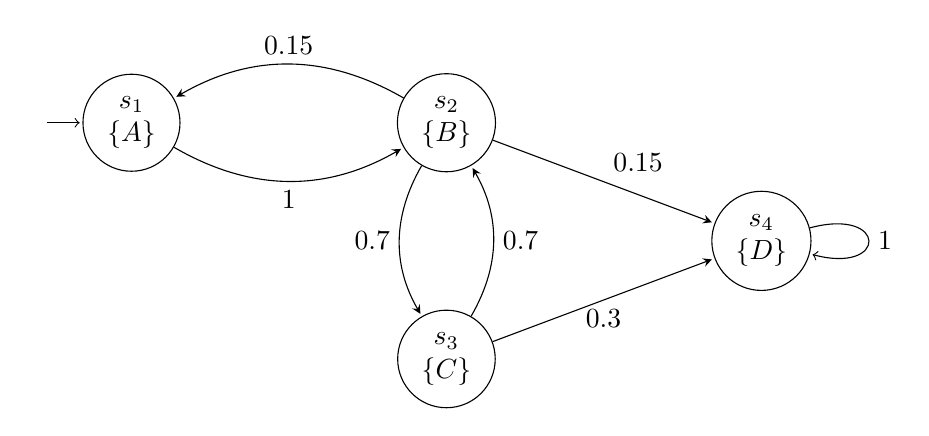
\begin{tikzpicture}[shorten >= 1pt, node distance=4cm, on grid, auto]
				\node[state, initial, initial text={}, align=center] (s_1) {$s_1$ \\ $\{A\}$};
				\node[state, align=center] (s_2) [right=of s_1] {$s_2$ \\ $\{B\}$};
				\node[state, align=center] (s_3) [below=of s_2, yshift=1cm] {$s_3$ \\ $\{C\}$};
				\node[state, align=center] (s_4) [right=of s_2, yshift=-1.5cm] {$s_4$ \\ $\{D\}$};
				
				\path[-stealth]
				(s_1) edge [bend right] node[below] {$1$} (s_2)
				(s_2) edge [bend right] node[above] {$0.15$} (s_1)
				(s_2) edge [bend right] node[left] {$0.7$} (s_3)
				(s_2) edge [] node {$0.15$} (s_4)
				(s_3) edge [bend right] node[right] {$0.7$} (s_2)
				(s_3) edge [] node[below] {$0.3$} (s_4)
				(s_4) edge [loop right] node {$1$} (s_4)
				;
			\end{tikzpicture}
			
			\caption{Graph für die Markov-Kette $\mathfrak{S}$}
			\label{MarkovGraph1}
		\end{center}
	\end{figure}
\end{example}

Bevor wir die Semantik von $\PCTL$-Formeln für Markov-Ketten formal definieren können benötigen wir noch den Begriff des Wahrscheinlichkeitsmaßes.

\begin{definition}[Wahrscheinlichkeitsmaß]
	 Sei $\pi = s_0\dots s_n$ eine Folge an Zuständen einer Markov-Kette $\mathfrak{S}$ und $X=\{\sigma\in \paths{\mathfrak{s}}{s_0} : \sigma\uparrow n = \pi\}$ die Menge aller (unendlichen) Pfade, die mit dieser Folge beginnen. Wir definieren dann das Wahrscheinlichkeitsmaß 
	 $$\mu^{\mathfrak{S}}_{s_0}(X)\coloneqq\mathcal{T}(s_0,s_1)\cdot \dots \cdot \mathcal{T}(s_{n-1},s_n)$$
	 als das Produkt der Kanten zwischen den Zustände der Folge.
\end{definition}

% Hinweis: Folge muss nicht explizit angegeben werden, da größter gemeinsamer Präfix von X verwendet werden kann und eindeutiges Ergebnis bringt -> Beweis
% Bemerkungen aus Skript

\begin{definition}[Semantik von $\PCTL$ auf Markov-Ketten]
	Sei $\mathfrak{S}=(S,s_i,\mathcal{T},\mathcal{L})$ eine Markov-Kette. Dann lässt sich die Semantik für $\PCTL$-Formeln induktiv definieren:
	\begin{enumerate}
		\item 
	\end{enumerate}
\end{definition}


\subsection{Semantik}

Hier wird die Semantik erklärt und das verwendete Transitionssystem, die Markov Kette eingeführt. 
Einige simple, abstrakte Beispiele ebenfalls zum Erklären verwendet werden.
Ein Vergleich mit $\CTL$ soll passieren, wobei auf die in \cite{hansson1994logic} definierte Einbettung verwiesen, aber auch der Fehler bzgl. $\operatorname{EG}\varphi$ gezeigt wird.

\subsection{Model-Checking Algorithmen}

Die in \cite{hansson1994logic} genannten Model-Checking Algorithmen werden erklärt und anhand von Tabellen und unterschiedlichen Formeln erläutert.
Wie im Paper soll eine Aufteilung in die unterschiedlichen Parameter-\textit{Arten} (also $0<t<\infty$, $t=0$, $t=\infty$ und analog für $p$) stattfinden.

\subsection{Angewandtes Beispiel}

Was genau als Beispiel verwendet wird, muss noch entschieden werden, im Zweifelsfall ein etwas anderes Übertragungsprotokoll als im Paper.
Einige unterschiedliche Formeln sollen übersetzt werden so, dass auch die Bedeutung anderer Formeln als nur $\leadsto$ klarer wird.

\section{Vergleich mit Halbringsemantik}

\emph{Ob dieses Kapitel umgesetzt wird hängt von der Vergleichbarkeit von Viterbi-Halbring + $\CTL$ mit $\PCTL$ ab. Der Platz im restlichen Teil der Arbeit, der durch die Existenz des Kapitels wegfällt, soll von Kapitel \ref{ChapVerwandt} gepuffert werden. Bei Platzproblemen kann über das Zusammenlegen der Kapitel \ref{HalbringFO} und \ref{HalbringCTL} nachgedacht werden.}
Hier soll kurz erklärt werden, was genau Halbringsemantik ist und wofür sie im Allgemeinen verwendet wird. In dieser Einleitung und Kapitel \ref{HalbringFO} wird vor allem auf \cite{gradel2017semiring} verwiesen.

\subsection{Halbringsemantik zum Auswerten von Wahrscheinlichkeiten}
\label{HalbringFO}

Verwendung des Viterbi-Halbrings zum Auswerten von $\mathsf{FO}$ auf Graphen. Dieses Kapitel wird bei Platzproblemen weggelassen und der Übergang von $\mathsf{FO}$ auf $\mathsf{CTL}$ wird kurz in Kapitel \ref{HalbringCTL} passieren. Falls ich kein veröffentlichtes Paper mit den Informationen finde, benutze ich \cite{gradel2022provenance}.

\subsection{Halbringsemantik für $\CTL$}
\label{HalbringCTL}

Erweiterung der Halbringsemantik für $\mathsf{FO}$ auf $\CTL$. Informationen sollen aus \cite{dannert2019generalized} und \cite{lluch2005quantitative} stammen.

\subsection{Vergleich von Halbringsemantik für $\CTL$ mit $\PCTL$}

Unterschiede im Ansatz der beiden Varianten. Falls sich diese einfach beheben lassen, Vergleich in der Nutzung, der Ausdruckskraft etc.

\section{Verwandte Arbeiten}
\label{ChapVerwandt}

Andere Ansätze die entweder nur Zeit oder Wahrscheinlichkeiten zu $\CTL$ bzw. Fixpunktlogiken hinzufügen sollen hier erläutert werden.

\subsection{Erweiterung von $\CTL$ durch Echtzeit}

Ein anderer Ansatz zum Ergänzen durch Zeit ist die in \cite{alur1990model} definierte Logik, welche erläutert werden soll. Interessant ist auch die Logik aus \cite{jahanian1986safety}, welche eine Fixpunkt-Logik, also ausdrucksstärker als $\CTL$ ist.
Ein Vergleich mit $\PCTL$ bzgl. der Ausdruckskraft soll folgen, evtl. mit Beschränkung von $p$ auf extreme Werte, also $p\in \{0,1\}$ für $\PCTL$.

\subsection{Erweiterung von $\CTL$ durch Wahrscheinlichkeiten}

Es gibt auch Logiken die nur Wahrscheinlichkeiten hinzufügen. Lassen sich unterschiedliche Ansätze finden? Lösen diese andere Probleme? Paper mit anderen probabilistischen Logiken (die $\CTL$ erweitern): \cite{hart1984probabilistic}, \cite{lehmann1982reasoning} und \cite{christoff1992reasoning}.

\section{Konklusion}

Hier fasse ich noch einmal kurz die Ergebnisse zusammen. Also was $\PCTL$ ist, wofür es benutzt werden kann und evtl. wie Halbringsemantik ein ähnliches Ergebnis erzielen kann.

\bibliography{references}

\end{document}
